\section{Inference}
\label{sec:soft-inference}
%
%
In this section the inference process is analyzed on the neural network model,
taking into account that the two applications share the same code. In fact, when
the model is loaded into the buffer, it is interpreted by the TensorFlow Lite
library, returning the training information of the model and in particular the
information regarding the input and output of the model.
For this case, where you are interested in the problem of object detection, the
size of the image is requested at the input and the number of color channels in
this case is constant and fixed at three.
Furthermore, the function reported in listing (\ref{lst:inference-support}) is
analyzed, which allows to adapt the model input with the data, that is, the
images coming from the camera, taking into account to satisfy the neural model
input and to adapt the information for the tensor calculation if in floating
point, or in 8-bit integers.
It also takes into account the process of quantization that took place during
the transformation from original model to lite model, in fact the input will
also be recalculated.
%
%
\begin{listing}[!h] 
\inputminted[frame=lines,framesep=2mm, linenos=true, autogobble, breaklines=true, fontsize=\scriptsize, firstline=29, lastline=70]{c++}{software/code/model_support_function.hpp} 
\caption{function that adapts the input image to the input required by the neural model.} 
\label{lst:inference-support} 
\end{listing}
%
%
For fully integer models, the inputs are unsigned integer 8-bit.\\ 
The mean and standard deviation (\texttt{std\_dev}), calculated as in
\eqref{eq:stddev}, values specify how to \texttt{uint8} values map to the float
input values used while training the model.\\
The mean is the integer value from $0$ to $255$ that maps to floating point
\texttt{$0.0\text{f}$}. 
\begin{equation}
\label{eq:stddev}
\text{\texttt{std\_dev}} = \frac{255}{\text{\texttt{float}}_\text{max}-\text{\texttt{float}}_\text{min}}
\end{equation}
Different hardware may have preferences and restrictions that may cause slight
deviations when implementing the specification that result in implementations
that are not bit-exact. Whereas that may be acceptable in most cases, the nature
of machine learning (and deep learning in the most common case) makes it
impossible to provide any hard guarantees.\cite{tflite-8bit}\\
8-bit quantization approximates floating point values using the following
formula \eqref{eq:8-bit}.
\begin{equation}
\label{eq:8-bit}
\text{\texttt{real}}_\text{\texttt{value}} = ({\text{\texttt{int8}}_\text{value}-\text{\texttt{zero}}_\text{point}}) \times \text{\texttt{scale}} 
\end{equation}
%
Per-axis (aka per-channel in Conv ops) or per-tensor weights are represented by
int8 two’s complement values in the range $[-127, 127]$ with zero-point equal to
0. Per-tensor activations/inputs are represented by \texttt{int8} two’s
complement values in the range $[-128, 127]$, with a zero-point in range $[-128,
127]$.
%
%
\subsection{Architecture x86\_64}
\label{ssec:x86-bench-inference}
We analyze in particular the inference cycle following the reception of the
frame by the TCP socket described previously in section
(\ref{ssec:software-coral-analysis}). It can be seen in figure
(\ref{subfig:all-bench}) that the captured process, where it is possible to
identify the functions performed:
\begin{itemize}
	\item The dark green rectangle represents the socket's reception function.
	\item The lighter green rectangle, on the other hand, is the time needed to calculate the inference.
	\item The pink rectangle represents the time to update the image in the user interface.
\end{itemize}
Although only one thread is shown here, in the solution adopted the TensorFLow
Lite module uses 8 cores, but it is possible to set a number of cores greater
than or equal to 1.
Comparing the two figures (\ref{subfig:time-cycle}) and
(\ref{subfig:time-inference}) it is observed that the duration of the cycle is
approximately $64.376 \,\si{\milli\second}$ and the other hand the infercence time
is $54.251 \,\si{\milli\second}$.
This time includes the execution of the functions described above, from this it
is possible to deduce that the most onerous task in terms of time and the
reconstruction of the image by the socket inside the
\textbf{TcpClient::imageAvailable} function. 
Meanwhile, \textbf{ModelTesnorFLowLite::run}'s function starts after about $10
\,\si{\milli\second}$ to end almost simultaneously with the function. Then the
cycle repeats itself.
Performing the inference with the TensorFlow Lite model, described in section
(\ref{sec:soft-inference}), on a laptop equipped with an Intel i7-7820HQ CPU
$2.90 \,\si{\giga\hertz}$ processor shows the benefits due to compression and
quantization of the neural model.
In particular, it is observed that the average time is $78 \,\si{\milli\second}$
therefore a considerable performance boost if compared with the time required,
when using the uncompressed model, is considerably slower when compared with the
result obtained in this case.
Although it is important to note that if the required time drops on the one
hand, the number of false positive cases increases on the other. 
%
\begin{figure}[htb]
	\centering
	\subfloat[][\emph{thread}.\label{subfig:all-bench}]%
		{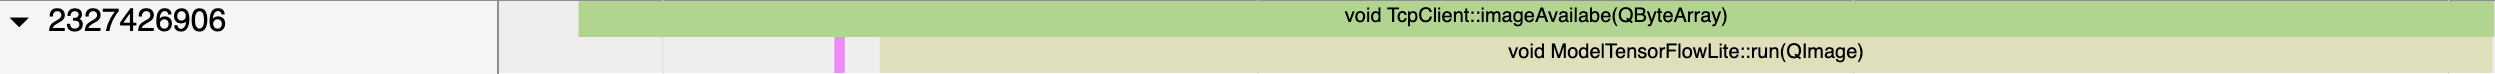
\includegraphics[width=\textwidth]{x86_64_1.jpg}} \\
	\subfloat[][\emph{time inference}.\label{subfig:time-inference}]%
		{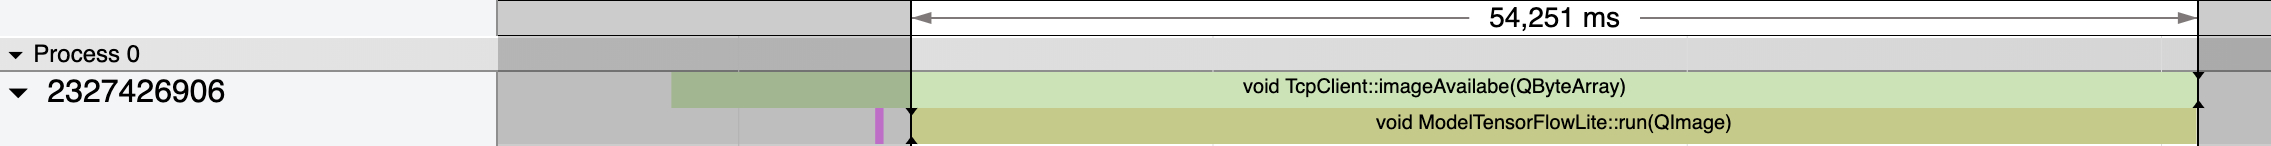
\includegraphics[width=\textwidth]{x86_64_2.jpg}} \\
	\subfloat[][\emph{total time cycle}.\label{subfig:time-cycle}]%
		{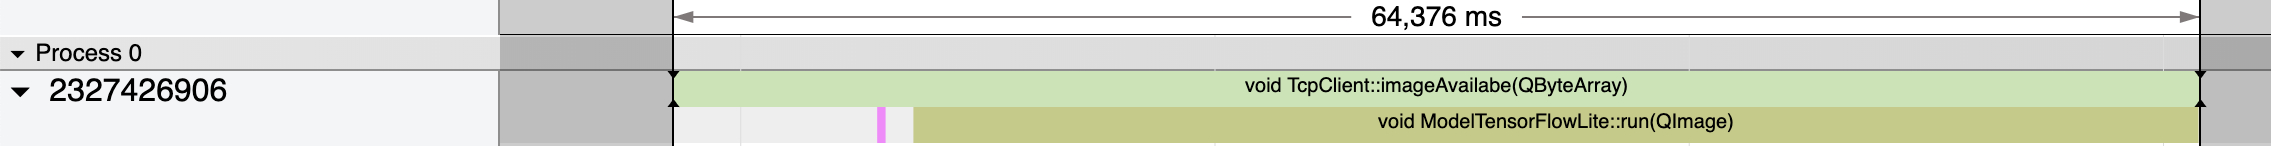
\includegraphics[width=\textwidth]{x86_64_3.jpg}}
	\caption{Visual benchmark inference on \texttt{x86\_64} architecture.}
	\label{fig:x86-bench}
\end{figure}
%
%
\subsection{Architecture armv7l}
\label{ssec:armv7l-bench-inference}
%
We now analyze the result of the execution of the inference process on the
hardware of the Raspberry Pi 3b computer board which mounts an ARM cortex-A53
processor.
In fact, the figures (\ref{fig:armv7l-bench}) show that the processes present a
different number and row, this is because parallel architecture is exploited and
in particular in the benchmark it has been possible to capture the distribution
of the tasks on the threads.
Unlike what is seen in the previous section, the inference is made immediately without
considering the expectation of the streaming of images by the socket.
The work cycle examined has a total duration of $694.296 \,\si{\milli\second}$,
please note that here too more than one core is assigned to the inference
process.
Moving forward in the analysis, we can distinguish within the cycle:
\begin{itemize}
	\item In green the image acquisition by the camera in the second thread.
	\item The orange rectangle the updating of the interface with the new image in the first thread.
	\item In bright green the execution of the function in the first thread that passes the image acquired by the camera to the function that performs the inference.
	\item The segment filled in olive green rectangle the inference process performed in the second thread.
\end{itemize}
As can be seen in figure (\ref{subfig:arm7-time-inference}), the inference process by the
\textbf{ModelTesnorFLowLite::run} function has an execution time of $528.105 
\,\si{\milli\second}$, considerably slower than the \texttt{x86\_64}
architecture previously discussed. although it has a longer execution time, the
whole program is not affected by this aspect due to the optimization carried out
by the compiler and by exploiting the multi-threading architecture as well as the
possibility of using SIMD\footnote{Single Instruction Multiple Data}
instructions.\\
Finally, we want to remember that both data come from the same code executed by
the machine, but two different architectures are being compared. 
The first encountered \texttt{x86\_64} supports 64-bit instructions, benefiting
from the larger size of the registers and in greater numbers, despite a much
higher clock frequency and being able to count on 4 physical and 4 virtual
cores. 
On the other hand the ARM process with \texttt{armv7l} architecture executes 32
bit instructions and has a much lower clock frequency.
%
\begin{figure}[htb]
	\centering
	\subfloat[][\emph{thread}.\label{subfig:arm7-all-bench}]%
		{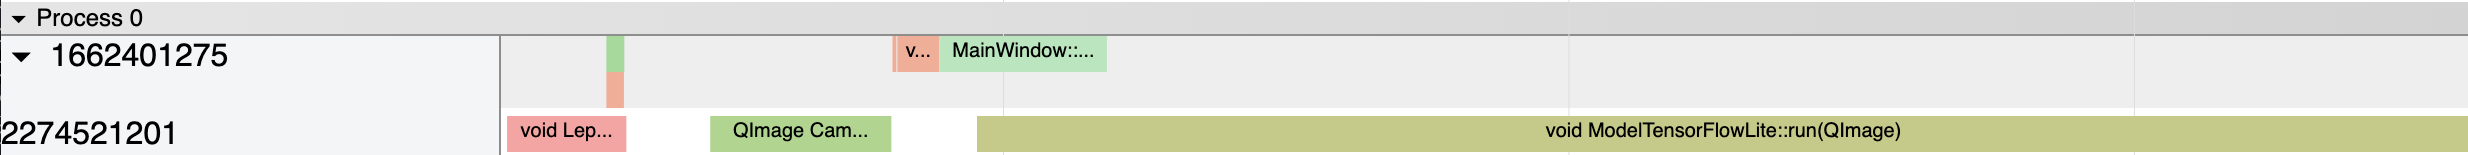
\includegraphics[width=\textwidth]{arm_32_1.jpg}} \\
	\subfloat[][\emph{time inference}.\label{subfig:arm7-time-inference}]%
		{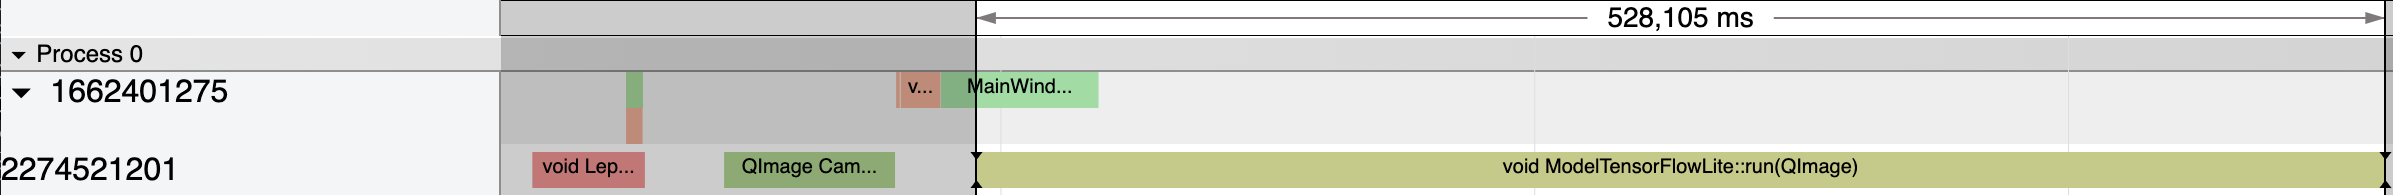
\includegraphics[width=\textwidth]{arm_32_2.jpg}} \\
	\subfloat[][\emph{total time cycle}.\label{subfig:arm7-time-cycle}]%
		{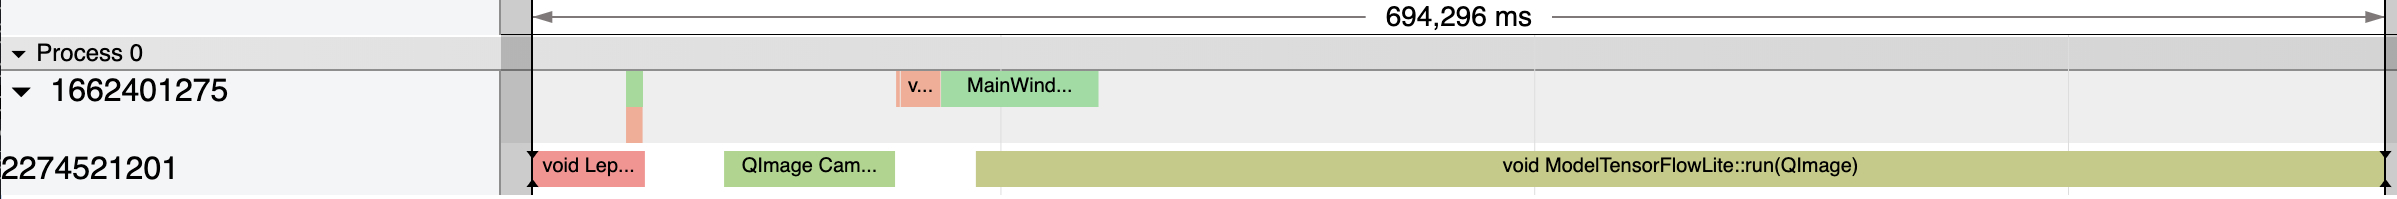
\includegraphics[width=\textwidth]{arm_32_3.jpg}}
	\caption{Visual benchmark inference on \texttt{armv7l} architecture.}
	\label{fig:armv7l-bench}
\end{figure}
%
\subsection{Architecture armv8a and TPU}
\label{ssec:tpu}
%
%
The last comparison is made on the processing capacity of Google's Coral
Dev-Board and in particular by the TPU that makes available for the tensor
calculation.
In the visual benchmark created in figure (\ref{subfig:TPU-all-bench}), unlike 
the previous ones, there is a single thread.
In this case it was not possible to isolate only the functions of interest, but 
all the calls to the functions made by the program were extracted.
In this analysis, unlike the previous ones, you are not using all the threads of
the processor that you remember is a 64-bit ARM cortex-A53.\\ 
The calculation is moved to the TPU thus relieving the main processor from the
calculation of the inference on the quantized model and compiled specifically to
operate on the unit.
Improvement can be observed with respect to the case of the execution of the
inference on the \texttt{armv7l} architecture in that when the times drop
drastically, in fact they are equal or better than to those seen in section
(\ref{ssec:x86-bench-inference}).\\  
The TPU processing unit performs the inference in approximately $36.317
\,\si{\milli\second}$ highlighted by the pink segment reported in figure 
(\ref{subfig:TPU-time-inference}) was called the \textbf{RunInference} 
function.
%
%
\begin{figure}[htb]
	\centering
	\subfloat[][\emph{thread}.\label{subfig:TPU-all-bench}]%
		{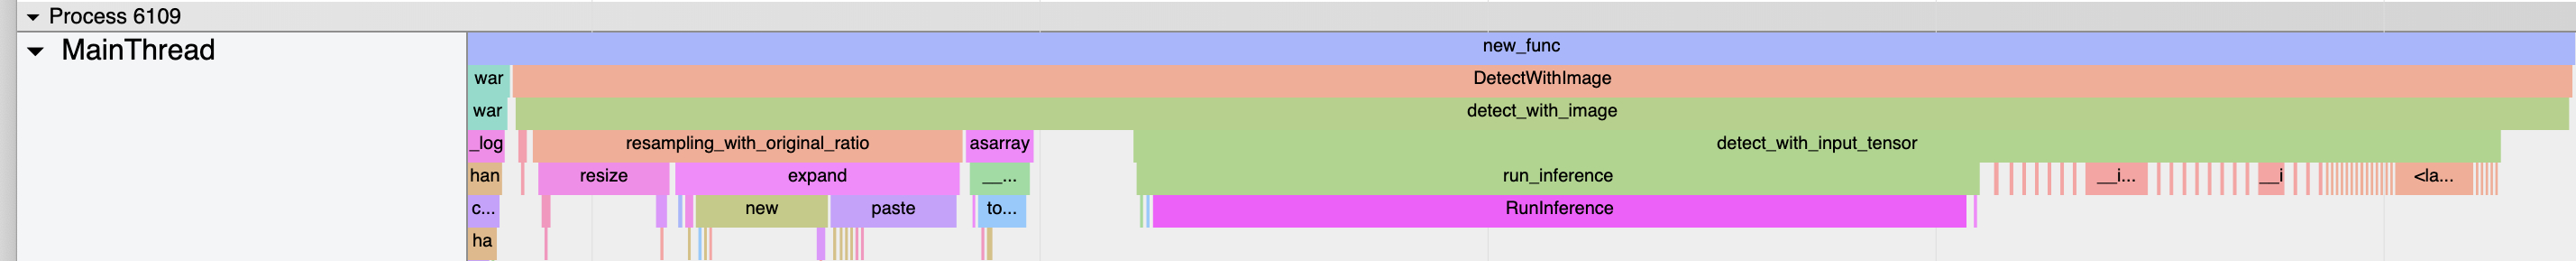
\includegraphics[width=\textwidth]{TPU_1.jpg}} \\
	\subfloat[][\emph{time inference}.\label{subfig:TPU-time-inference}]%
		{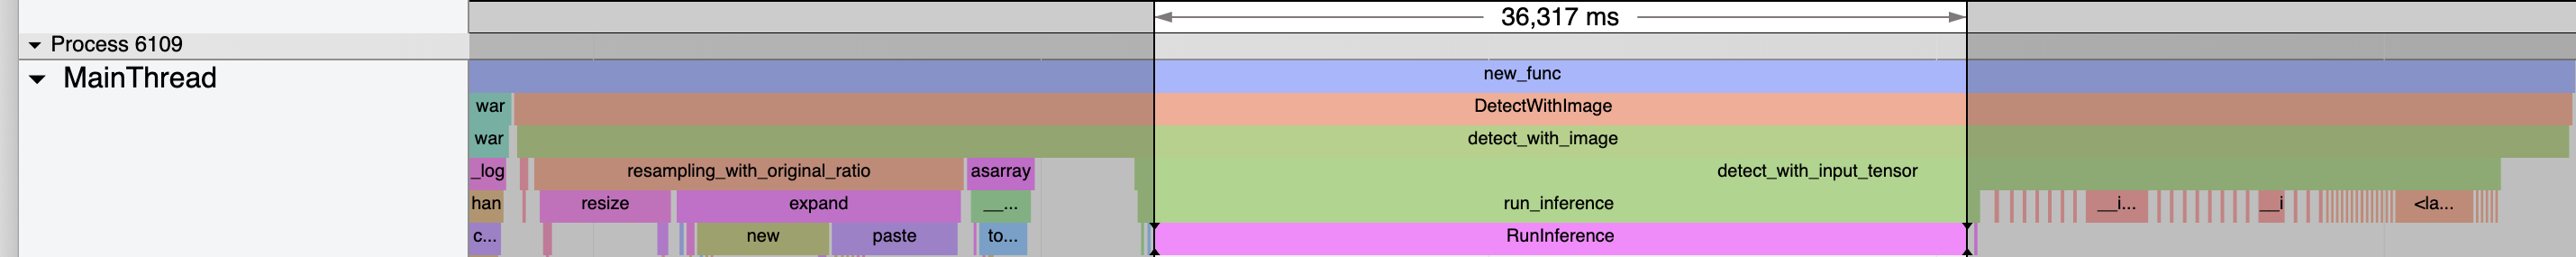
\includegraphics[width=\textwidth]{TPU_2.jpg}} \\
	\subfloat[][\emph{total time cycle}.\label{subfig:TPU-time-cycle}]%
		{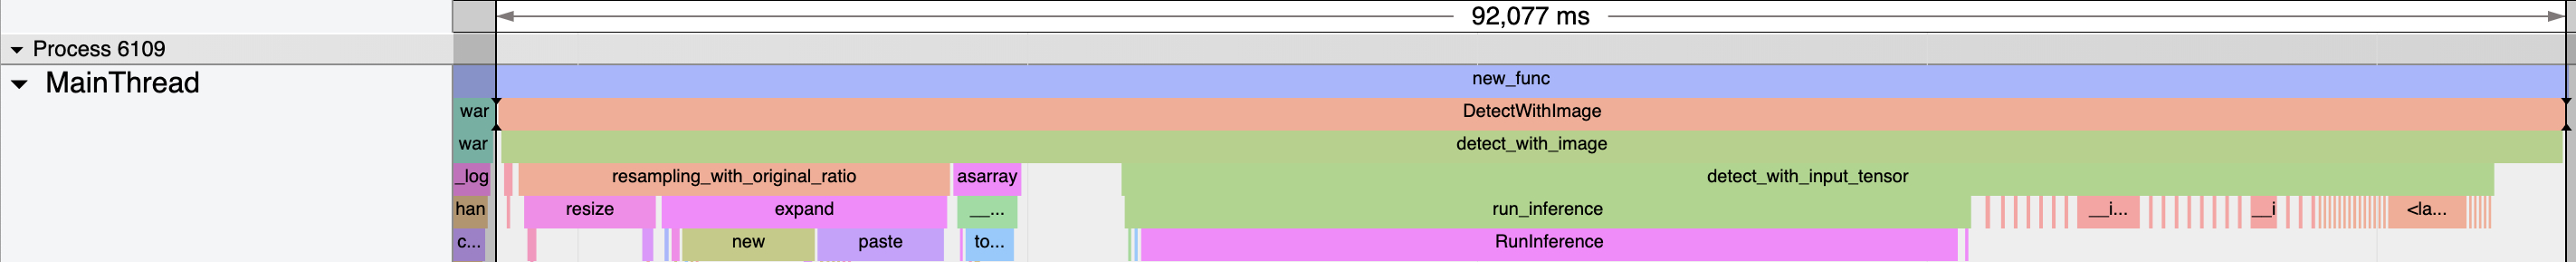
\includegraphics[width=\textwidth]{TPU_3.jpg}}
	\caption{Visual benchmark inference on \texttt{TPU}.}
	\label{fig:TPU-bench}
\end{figure}

As seen in (\ref{sec:hard-tpu}), the advantage of using TPU to perform largely derives
from the adoption of 8-bit integers that make tensor calculation easier.\\
Furthermore, the structure of the systolic array also guarantees benefits due to
the possibility of keeping the calculation time constant as the tensor
increases.
The entire inference calculation cycle is $92.077 \, \si{\milli\second}$ in
which the image arrives. The image is scaled to the desired input of the tensor
and ready to be analyzed, as observable in figure (\ref{subfig:TPU-time-cycle}).
